\chapter{STP Tree Generator}
\label{stp_gen}
Our STP Tree Generator itself is made up of three different executables:
The client uses the data from the received BPDUs and combines them into its path to the root.
The server registers the clients and stores their information.
It also takes care of removing information from clients that stopped sending data, because it has to be assumed that these clients have been disconnected along with the bridges they were connected to.
The last executable is the so-called parser, which is used to obtain the finished report.
It connects to the server with a special message, causing the server to combine the data from the different clients.
Afterwards it will parse the combined data to a \textit{.tikz} file.
\section{Setup}
The intended way of using this tool is having multiple clients connect to a central server.
If there is a client connected to every bridge in the network, all of them will be in the report.
However, this does not mean that all connections are in the report as well, as connection information can only be obtained during tree buildup (see Section~\ref{packet_handling}).
An example setup can be seen in Figure~\ref{fig:example_setup}.
In general it is advisable to place the clients more towards the bottom of the tree.
This way there is a chance to obtain information on intermediate bridges, should a tree buildup be observed by the client.
Where the server is placed is irrelevant, as long as connectivity is ensured.

\begin{figure}[h]
    \centering
    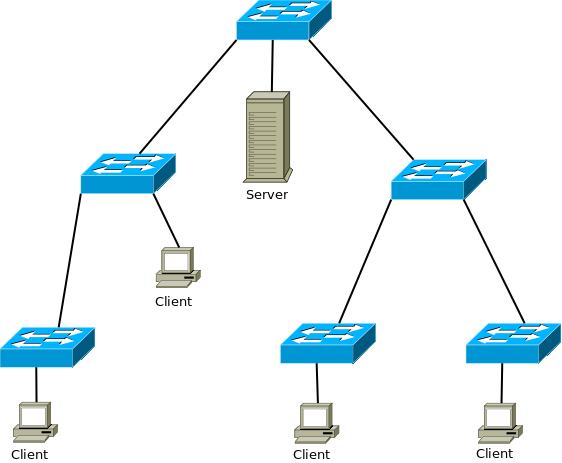
\includegraphics[width=0.7\textwidth]{example_setup.png}
    \caption{An example STP tree generator setup}
    \label{fig:example_setup}
\end{figure}

\section{Client-Server Communication}
For the communication we used Transmission Control Protocol (TCP) sockets.
TCP was used because it utilizes sessions, and takes care of guaranteeing correct transmission of the data.
Alternatively we could have used the User Datagram Protocol (UDP), which would have saved network traffic needed for establishing the TCP connection, but would have required us to implement some sort of message acknowledgement scheme.
There are three different message types in packages:
\begin{enumerate}
    \item \textbf{register}: Clients send these to the server in order to receive a new unique identifier.
    \item \textbf{push}: Clients send these packets when they push new tree information to the server.
        These packets are sent every time a client receives an STP packet.
    \item \textbf{report}: The parser sends this message type when requesting a visualization.
\end{enumerate}
The ids are used by the server to identify push messages sent by the different clients.
They are also used to identify clients that are not sending new packets.
Information from these clients is then removed.
After it has registered, the client will then send "push" packets to the server.
These contain the path information in JSON format, as well as the id.
Push packets will be sent by the client every time they receive an STP packet.
If the parser is called, it will send a "report" package to the server, causing it to combine the client data to into trees and sending them back to the parser.
